% This is a LaTeX thesis template for Monash University.
% to be used with Rmarkdown
% This template was produced by Rob Hyndman
% Version: 6 September 2016

\documentclass{monashthesis}

%%%%%%%%%%%%%%%%%%%%%%%%%%%%%%%%%%%%%%%%%%%%%%%%%%%%%%%%%%%%%%%
% Add any LaTeX packages and other preamble here if required
%%%%%%%%%%%%%%%%%%%%%%%%%%%%%%%%%%%%%%%%%%%%%%%%%%%%%%%%%%%%%%%

\author{Weihao Li}
\title{Using Remote Sensing Data to Understand Fire Ignition during the
2019-2020 Australia Bushfire Season}
\studentid{28723740}
\def\degreetitle{Bachelor of Commerce (Honours)}
% Add subject and keywords below
\hypersetup{
     %pdfsubject={The Subject},
     %pdfkeywords={Some Keywords},
     pdfauthor={Weihao Li},
     pdftitle={Using Remote Sensing Data to Understand Fire Ignition during the
2019-2020 Australia Bushfire Season},
     pdfproducer={Bookdown with LaTeX}
}


\bibliography{thesisrefs}

\begin{document}

\pagenumbering{roman}

\titlepage

{\setstretch{1.2}\sf\tighttoc\doublespacing}

\clearpage\pagenumbering{arabic}\setcounter{page}{0}

\chapter{Statement of the topic}\label{ch:intro}

Along with the extreme heatwave in Australia 2019-2020, one of the most
devastating bushfire season in history had been witnessed. Lighting
strikes and arson were been discussed among pubilc as the main cause of
this disaster. This research will explore the methods of fire ignition
during 2019-2020 Australia bushfires season and provide a model to
predict the fire risk of neighbourhoods. Hotspots data from the JAXA's
Himawari-8 satellite and weather data from the Australian Bureau of
Meteorology will be used in ignition identification and bushfire danger
estimation. In addition, an interactive web application embeds with
research outcomes will be built for data visualization purpose.

\section{Motivation}\label{motivation}

\textless{}left blank\textgreater{}

\section{Research aim and questions}\label{research-aim-and-questions}

This research aims to answer the following questions:

\begin{enumerate}
\def\labelenumi{\arabic{enumi}.}
\tightlist
\item
  How to find the ignition methods during 2019-2020 Australia bushfire
  season?
\item
  How to model fire risk of neighbourhoods?
\end{enumerate}

\section{Research plan}\label{research-plan}

\textless{}left blank\textgreater{}

\section{Scope of research}\label{scope-of-research}

\textless{}left blank\textgreater{}

\chapter{Literature Review}\label{literature-review}

\textless{}left blank\textgreater{}

\chapter{Data collection and
processing}\label{data-collection-and-processing}

In order to answer the reserach questions, this research will use
mutiple geospatial datasets and weather datasets.

\section{Sources}\label{sources}

Two methods were performed to collect necessary datasets, including
retrieve files from servers and crawl data from websites. For
reproducibility purpose, only public data will be used in this research.

To obtain fire history, we used the hotspots data from JAXA's Himawari-8
satellite. This satellite is positioned in geostationary orbit at 140
degrees east longitude, and the revisit period is 10-minute. Its
management system - JAXA's P-Tree system, provides WildFire observation
product with 2km spatial resolution. (P-Tree System, 2020).

Weather data were collected from the Australian Bureau of Meteorology,
by using an R package - Bomrang. Due to the limitation of APIs provided
by the package, we crawled data from BOM's website for extra
information.

To characterise the fuel we used forest of Australia (2018) from the
Australian Bureau of Agriculture and Resource Economics and Sciences. It
is a fuel layer contains the vegetation information across Australia.

Information on the datasets not covered above can be found in Table
\ref{tab:datasetinfo}.

\begin{table}[t]

\caption{\label{tab:datasetinfo}Data information}
\centering
\fontsize{9}{11}\selectfont
\begin{tabular}{llll}
\toprule
Data set name & Spatial Resolution & Temporal resolution & Time\\
\midrule
Hotspots data - JAXA’s Himawari-8 satellite & $0.02^\circ \approx 2km$ & Per 10 minutes & 2015-2020\\
Weather data - Australian Bureau of Meteorology &  & Daily & 2019-2020\\
Map - OpenStreetMap & 2m &  & 2020\\
Fuel layer - Australian Bureau of Agriculture \\ $\hspace{5mm}$ and Resource Economics and Sciences & 100m &  & 2018\\
Victorian CFA fire stations - Department of Environment, \\ $\hspace{5mm}$Land, Water $\&$ Planning & 20m &  & 2020\\
\addlinespace
Victorian Recreation sites - Department of Environment, \\ $\hspace{5mm}$Land, Water $\&$ Planning & 10m &  & 2020\\
\bottomrule
\end{tabular}
\end{table}

\section{Pre-processing}\label{pre-processing}

An R package sf (Edzer, 2020) has been used to convert all geospatial
data into simple features. We then used Tidyverse (Hadley et al., 2020)
as a data wrangling tool to manipulate data.

To preprocess the hotspots data, we selected the observations in
Australia from the full disk. Meanwhile, hotspots with irradiance under
100 watt per square metre will be deleted. We restricted our study to
hotspots that have significant firepower. An hour id has been assigned
to each observation range from 1 to T, represents the relative time the
hotspot being observed. On top of the tidy hotspots data, a clustering
algorithm was developed to identify fire clusters. Details about the
algorithm can be found in table \ref{tab:clustering}.

By using this algorithm, we assigned each hotspot a cluster membership
which we called \emph{fire\_id}. Meanwhile, we recorded the
characteristics of each cluster including its centroid, starting time,
ending time and movement. The inspiration behind this algorithm is the
real world bushfire behaviour which can be summarised as two
hyperparameters, the distance of spread in each hour and the lifetime of
fire since it not being detected, represented by \(r_0\) and \(t_0\)
respectively. These two hyperparameters have been used to determine if a
new hotspot belongs to an existing or new cluster.

\newpage

\normalfont

\begin{table}
\caption{\label{tab:clustering}A clustering algorithm for hotspots}
\begin{align*}
&\rule{150mm}{0.5mm}\\[-1\jot]
&\textbf{Algorithm 1 Hotspots clutering}\\[-1\jot]
&\rule{150mm}{0.5mm}\\[-1\jot]
&\textbf{input: }~~~~\text{Hotspots dataset H : (Hour}\textunderscore \text{id}^{(n)} \text{, Coordinates}^{(n)} \text{), n = 1, 2, ... N}\\[-1\jot]
&~~~~~~~~~~~~~~~~\text{An empty dataset F : (Fire\textunderscore id}^{(m)} \text{, Coordinates}^{(m)} \text{, Active}^{(m)} \text{), m = 1, 2, ...}\\[-1\jot]
&~~~~~~~~~~~~~~~~\text{An empty vector K} \in \mathbb{N}_1^n\\[-1\jot]
&~~~~~~~~~~~~~~~~\text{A distance hyperparameter }r_0 \in \mathbb{R}^+\\[-1\jot]
&~~~~~~~~~~~~~~~~\text{A time hyperparameter }t_0 \in \mathbb{N}^+\\[-1\jot]
&\textbf{output: }~~\text{A vector K} \in \mathbb{N}_1^n~\text{contains memberships of hotspots}\\[-1\jot]
&~~~~~~~~~~~~~~~~\text{A dataset F contains fire clusters information including memberships, latest}\\[-1\jot]
&~~~~~~~~~~~~~~~~\text{centroids and time from last updated}\\[-1\jot]
&~~1:~~\text{select subset }H_c \in \text{H where Hour\textunderscore id == 1}\\[-1\jot]
&~~2:~~\text{calculate distance matrix D for Coordinates in }H_c \\[-1\jot]
&~~3:~~\text{assign 1 to a zero adjacency matrix A for where D} \leq r_0~~//~~\text{hotspots with relative}\\[-1\jot]
&~~~~~~~~~\text{distance less or equal to }r_0~\text{will be considered belong to the same cluster} \\[-1\jot]
&~~4:~~\text{create undirected unweighted graph G from A}\\[-1\jot]
&~~5:~~\text{record memberships of G to K}\\[-1\jot]
&~~6:~~\text{record clusters classes to Fire\textunderscore id and record clusters centroids to Coordinates of F}\\[-1\jot]
&~~7:~~\text{set Active in F to }t_0~~//~~\text{Active clusters are fire being observed in the last }t_0~\text{hour}\\[-1\jot]
&~~8:~~\textbf{for}~~\text{hour = 2, ... T}~~\textbf{do} \\[-1\jot]
&~~9:~~~~~~~~\text{let Active -1 and select subset }F_c \in \text{F where Active} \geq 0\\[-1\jot]
&10:~~~~~~~~\text{select subset }H_c \in \text{H where Hour\textunderscore id == hour}\\[-1\jot]
&11:~~~~~~~~\text{append Coordinates from }F_c~\text{to}~H_c\\[-1\jot]
&12:~~~~~~~~\text{repeat step 2 - 4}\\[-1\jot]
&12:~~~~~~~~\textbf{for}~~h_i = \text{each hotspot in }H_c~~\textbf{do}\\[-1\jot]
&13:~~~~~~~~~~~~~~\textbf{if}~~h_i~\text{share the same membership as one of active clusers in }F_c~~\textbf{then}\\[-1\jot]
&14:~~~~~~~~~~~~~~~~~~~~\text{copy the corresponding Fire\textunderscore id of the nearest active cluser to K}\\[-1\jot]
&15:~~~~~~~~~~~~~~\textbf{else}~~\text{copy the membership from G to K}\\[-1\jot]
&16:~~~~~~~~~~~~~~\textbf{end if}\\[-1\jot]
&17:~~~~~~~~\textbf{end for}\\[-1\jot]
&18:~~~~~~~~\text{update F for clusters involed in current timestamp and reset corresponding}\\[-1\jot]
&~~~~~~~~~~~~~~~\text{Active to }t_0\\[-1\jot]
&19:~~\textbf{end for}\\[-1\jot]
&\rule{150mm}{0.5mm}
\end{align*}
\end{table}

\section{Conceptual Entity Relationship
Diagram}\label{conceptual-entity-relationship-diagram}

In Figure \ref{fig:ERD}, we present the conceptual entity relationship
diagram for the data model will be used in both data modelling and shiny
app development.

\begin{figure}
\centering
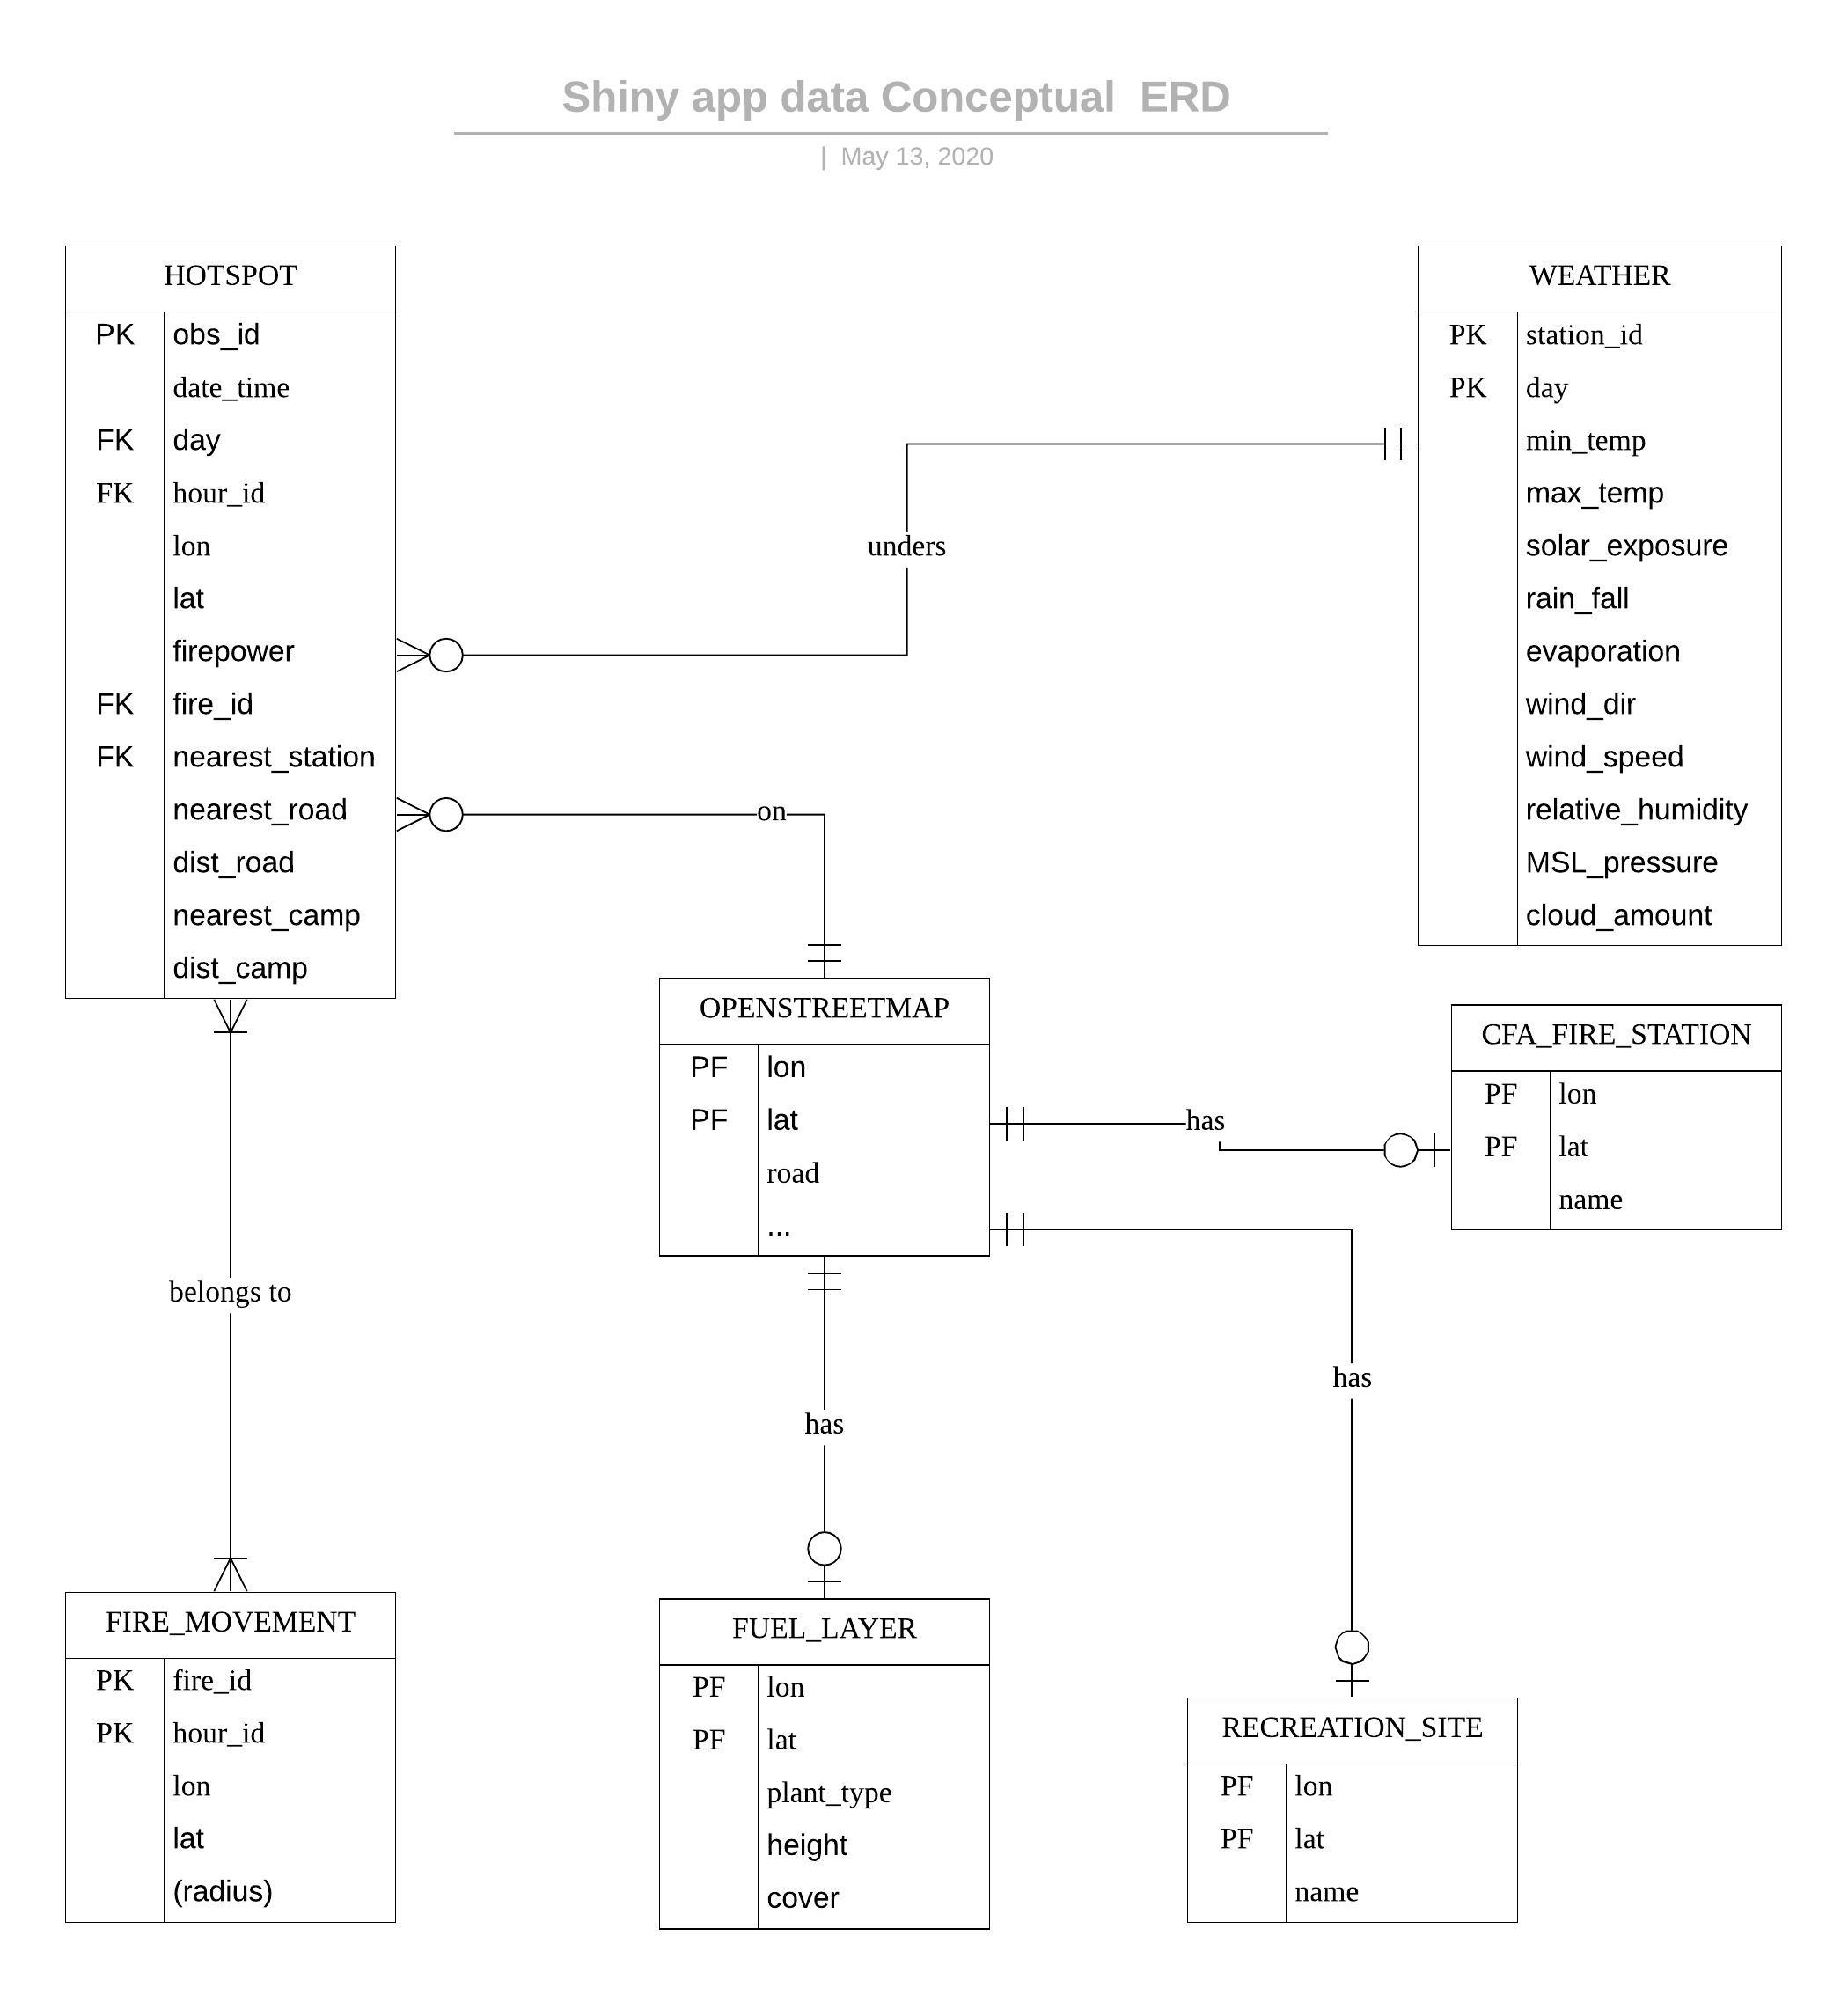
\includegraphics{figures/Shiny_app_data_Conceptual_ERD.jpeg}
\caption{Conceptual ERD for the shiny app data model \label{fig:ERD}}
\end{figure}

\chapter{Exploratory data analysis}\label{exploratory-data-analysis}

\chapter{Modelling}\label{modelling}

\textless{}plan\textgreater{}

\section{Predicting ignition method}\label{predicting-ignition-method}

\textless{}plan\textgreater{}

\section{Modelling fire risk}\label{modelling-fire-risk}

\textless{}plan\textgreater{}

\chapter{Timeline}\label{timeline}

The research plan for this semseter can be found in Table
\ref{tab:timeline1}. Future research plan can be found in Table
\ref{tab:timeline2}.

\begin{table}[!h]

\caption{\label{tab:timeline1}Research plan till week 9}
\centering
\begin{tabular}{ll}
\toprule
Timeline & Tasks\\
\midrule
Week 2 & Geographic data background reading\\
Week 3 & Collect Remote sensing data (JAXA himawari-8 satellite) and\\
 & explore BOM weather data APIs (Bomrang)\\
Week 4 & Collect Road Map (OpenStreetMap) and\\
 & read articles in SpatioTemporal data visualization and modelling\\
\addlinespace
Week 5 & Develop clustering algorithm for remote sensing data\\
Week 6 & Test diferent hyperparameters for clusetring\\
Week 7 & Exploratory data analysis on fire clusters and data integration\\
Week 8 & Feature planning for the shiny app\\
week 9 & Write research proposal and prepare the first presentation\\
\bottomrule
\end{tabular}
\end{table}

\begin{table}[!h]

\caption{\label{tab:timeline2}Research plan since June}
\centering
\begin{tabular}{ll}
\toprule
Timeline & Tasks\\
\midrule
June - July & Modelling fire ignition and fire risk\\
August & Consolidate findings and create mockups of the shiny app\\
September & Develop the shiny app and perform different levels of testing\\
October & Write thesis and prepare the second presentation\\
\bottomrule
\end{tabular}
\end{table}

\chapter{Supplementary materials}\label{supplementary-materials}

\chapter{Biblography}\label{biblography}

\chapter{Words from last week}\label{words-from-last-week}

\section{Data}\label{data}

\section{Methodology}\label{methodology}

Both supervised and unsupervised learning will be implemented to reach
the research aims.

To understand the ignition of bushfires, a customized clustering
algorithm will be developed to convert hotpots data into fire history,
which will contain the starting time and coordinates of each fire. This
algorithm will mainly involve simulating fire growth, deciding fire
boundaries controlled by tolerance and assigning hotspots data to the
most probable cluster. After the clustering result being obtained, fire
history will be visualized to diagnostic the performance of the
algorithm. It will be done by comparing the behaviour of the same fire
under different sets of hyperparameters.

Exploratory data analysis of fire history and its relative factors, like
weather condition, distance to the nearest road and distance to the
nearest recreation site will be performed. Prior knowledge and featuring
engineering will be needed to fully understand the relationship. We
expect to discover relationships between the ignition of fire with these
factors, which can help us identify the cause of bushfires later on.

In order to examine the sources of fire ignition, different strategies
will be used depending on the outcome in the previous section. If the
findings from the analysis are strong and directly related to potential
sources of fire ignition, hypothesis tests will be conducted to examine
the pattern. If the evidence is weak, we will consider developing
another clustering algorithm on fire history. This algorithm will be
designed to maximize the distance between bushfire started with
different causes in a high dimensional space. A probability model then
can be built on top of it, which can provide a probabilistic answer for
the source of bushfire ignition during 2019-2020 bushfire season.

Models for predicting fire risk of neighbourhoods will be built using
raw hotspots data instead of the fire history because the hotspots data
can be considered generated from a partially observable Markov decision
process, and the underlying state is the development of the bushfire.
From low complexity models like logistic regression to high complexity
models like deep neural network will be tested.

For sharing our research outcome, a shiny app will be built and hosted
online. In addition, both static and dynamic visualization tools will be
considered using. Due to the nature of Spatio-temporal data, which has
at least 3-dimensional features, static map view without faceting can
only provide limited information. Meanwhile, faceting map view with time
will be limited by the size of caravans. Animation based map view is
computationally expensive and distracting though it provides more
information. Better ways for visualizing Spatio-temporal data will be
explored during the development. The potential product will be an
interactive map view with triggers to transform data and manipulate the
aesthetics specifications.

\section{Preliminary Results}\label{preliminary-results}

\appendix

\chapter{Additional stuff}\label{additional-stuff}

You might put some computer output here, or maybe additional tables.

Note that line 5 must appear before your first appendix. But other
appendices can just start like any other chapter.

\printbibliography[heading=bibintoc]



\end{document}
